\section{Technical Method}
\label{sec:technical_method}

\begin{figure*}[t]
    \centering
    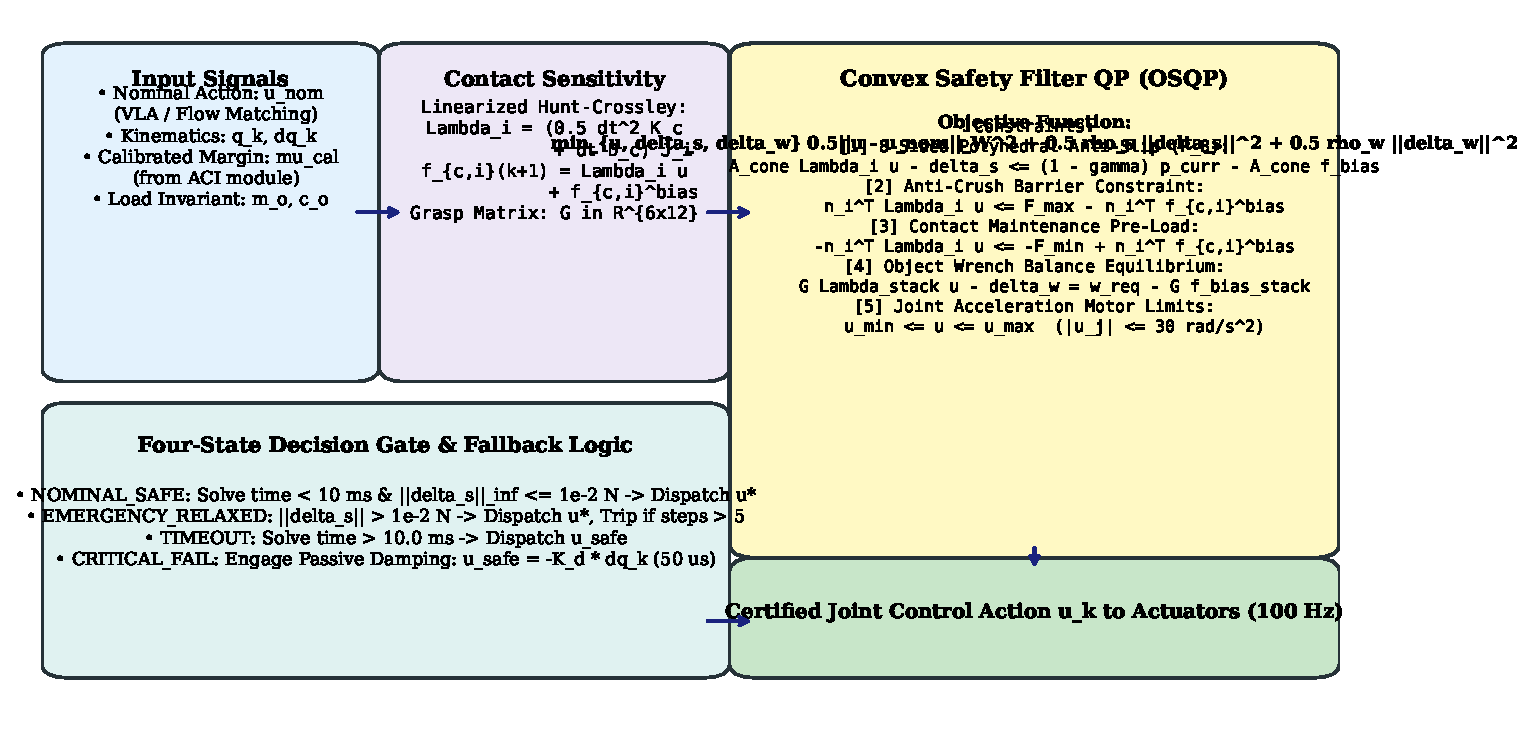
\includegraphics[width=\textwidth]{figures/safety_filter_diagram.pdf}
    \caption{\textbf{Predictive Safety Filter and Real-Time Decision Gate (Figure 2).} Detail of the OSQP optimization structure, integrating the 8-sided polyhedral anti-slip barrier, anti-crush force ceiling, grasp wrench equilibrium, four-state supervisor, and passive damping fallback.}
    \label{fig:safety_filter_detail}
\end{figure*}

\subsection{Multi-Contact State and Load Invariant Estimation}
At each control step $k$, optical tactile deformation is decoupled into normal pressure distribution and tangential shear traction fields across the sensor array. The normal contact force $f_{N, i}$ is obtained by integrating the normal stress profile, while tangential shear force $\mathbf{f}_{T, i} \in \mathbb{R}^2$ is computed from surface marker displacements.

Given the spatial contact forces $\mathbf{f}_{c, i} = f_{N, i} \hat{\mathbf{n}}_i + \mathbf{f}_{T, i}$ and contact locations $\mathbf{p}_{c, i}$, the net gravitational load and Center of Mass are tracked via recursive least-squares (RLS) with exponential forgetting factor $\lambda_{\text{rls}} = 0.98$:
\begin{align}
    \hat{m}_o(k) &= \frac{1}{g} \left\| \sum_{i=1}^M \mathbf{f}_{c, i}(k) \right\|_2 \\
    \hat{\mathbf{c}}_o(k) &= \left( \sum_{i=1}^M f_{N, i}(k) \mathbf{p}_{c, i} \right) \Bigg/ \left( \sum_{i=1}^M f_{N, i}(k) \right)
\end{align}
The instantaneous apparent friction coefficient is estimated via the tangential traction ratio:
\begin{equation}
    \hat{\mu}_i(k) = \frac{\|\mathbf{f}_{T, i}(k)\|_2}{f_{N, i}(k) + \epsilon}
\end{equation}

\subsection{Adaptive Conformal Inference (ACI) Module}
Standard friction estimators output point estimates $\hat{\mu}_i(k)$ that lag behind physical reality during sudden nonstationary drops (e.g., oil spills or condensation). Rather than asserting heuristic safety factors, we deploy Adaptive Conformal Inference (ACI) \cite{gibbs2021adaptive}.

Let $\alpha \in (0, 1)$ denote the target miscoverage rate (set to $\alpha = 0.05$ for certified $95\%$ coverage). At step $k$:
\begin{enumerate}
    \item \textbf{Non-Conformity Scoring:} We compute the absolute residual:
    \begin{equation}
        E_k = |\mu_{\text{observed}, i}(k) - \hat{\mu}_i(k)|
    \end{equation}
    \item \textbf{Online Quantile Tracking:} The adaptive parameter $\alpha_t$ updates via Robbins-Monro stochastic approximation:
    \begin{equation}
        \alpha_{t+1} = \alpha_t + \beta \left( \alpha - \mathbb{I}\{E_t > Q_t\} \right)
        \label{eq:aci_update_rule}
    \end{equation}
    where $\beta = 0.05$ is the adaptation rate, $\mathbb{I}\{\cdot\}$ indicates miscoverage, and $Q_t = \text{Quantile}_{1 - \alpha_t}(E_{1:t-1})$.
    \item \textbf{Calibrated Lower Bound:} The friction coefficient passed to the cone constraints is:
    \begin{equation}
        \mu_{\text{cal}, i}(k) = \max\left( \mu_{\text{floor}}, \hat{\mu}_i(k) - Q_{1 - \alpha_{t+1}}(E_{1:t}) \right)
        \label{eq:mu_cal_bound}
    \end{equation}
    where $\mu_{\text{floor}} = 0.05$ guarantees physical non-negativity.
\end{enumerate}

\subsection{Convex Quadratic Programming Formulation}
The safe joint acceleration command $\mathbf{u}^* \in \mathbb{R}^{n_q}$ is resolved at each $100\text{ Hz}$ control cycle via the following convex QP:
\begin{equation}
    \min_{\mathbf{u}, \boldsymbol{\delta}_s, \boldsymbol{\delta}_w} \frac{1}{2} \|\mathbf{u} - \mathbf{u}_{\text{nom}}\|_{\mathbf{W}}^2 + \frac{1}{2} \rho_s \|\boldsymbol{\delta}_s\|_2^2 + \frac{1}{2} \rho_w \|\boldsymbol{\delta}_w\|_2^2
    \label{eq:full_qp_filter}
\end{equation}
\textbf{Subject to:}
\begin{align}
    \mathbf{A}_{\text{ineq}} \mathbf{u} - \boldsymbol{\delta}_s &\le \mathbf{b}_{\text{ineq}} \label{eq:qp_ineq_sys} \\
    \mathbf{A}_{\text{eq}} \mathbf{u} - \boldsymbol{\delta}_w &= \mathbf{b}_{\text{eq}} \label{eq:qp_eq_sys} \\
    \boldsymbol{\delta}_s \ge \mathbf{0}, \quad \mathbf{u}_{\min} &\le \mathbf{u} \le \mathbf{u}_{\max} \label{eq:qp_bounds_sys}
\end{align}

Here, $\mathbf{W} = \mathbf{I}_{n_q}$. Soft slack variables $\boldsymbol{\delta}_s \in \mathbb{R}^{8M + 2M + 2n_q}$ and $\boldsymbol{\delta}_w \in \mathbb{R}^6$ ensure continuous recursive feasibility. Penalties are set to $\rho_s = 10^5$ and $\rho_w = 10.0$, strictly penalizing barrier violations while permitting compliant adjustment in net wrench balance.

The constraint matrices aggregate the multi-contact dynamics:
\begin{equation}
    \mathbf{A}_{\text{ineq}} = \begin{bmatrix}
        \mathbf{A}_{\text{cone}, 1} \mathbf{\Lambda}_1 \\
        \vdots \\
        \mathbf{A}_{\text{cone}, M} \mathbf{\Lambda}_M \\
        \hat{\mathbf{n}}_1^T \mathbf{\Lambda}_1 \\
        \vdots \\
        -\hat{\mathbf{n}}_M^T \mathbf{\Lambda}_M \\
        \mathbf{I}_{n_q} \\
        -\mathbf{I}_{n_q}
    \end{bmatrix}, \quad
    \mathbf{b}_{\text{ineq}} = \begin{bmatrix}
        (1 - \gamma_{\text{slip}}) \mathbf{p}_{\text{curr}, 1} - \mathbf{A}_{\text{cone}, 1} \mathbf{f}_{c, 1}^{\text{bias}} \\
        \vdots \\
        (1 - \gamma_{\text{slip}}) \mathbf{p}_{\text{curr}, M} - \mathbf{A}_{\text{cone}, M} \mathbf{f}_{c, M}^{\text{bias}} \\
        F_{\max} - \hat{\mathbf{n}}_1^T \mathbf{f}_{c, 1}^{\text{bias}} \\
        \vdots \\
        -F_{\min} + \hat{\mathbf{n}}_M^T \mathbf{f}_{c, M}^{\text{bias}} \\
        \mathbf{u}_{\max} \\
        -\mathbf{u}_{\min}
    \end{bmatrix}
\end{equation}
and $\mathbf{A}_{\text{eq}} = \mathbf{G} \mathbf{\Lambda}_{\text{stack}}$, $\mathbf{b}_{\text{eq}} = \mathbf{w}_{\text{req}} - \mathbf{G} \mathbf{f}_{\text{bias, stack}}$.

\begin{algorithm}[t]
\caption{Predictive Safety Filter Execution Loop ($100\text{ Hz}$)}
\label{alg:safety_filter}
\begin{algorithmic}[1]
\REQUIRE Nominal action $\mathbf{u}_{\text{nom}}$, joint state $(\mathbf{q}_k, \dot{\mathbf{q}}_k)$, tactile afferents $\mathbf{f}_{c, i}(k)$, target miscoverage $\alpha = 0.05$.
\ENSURE Safe joint acceleration command $\mathbf{u}_k^*$.
\STATE Ingest tactile shear and normal forces; detect incipient slip marker divergence.
\STATE Update load invariants $(\hat{m}_o, \hat{\mathbf{c}}_o)$ and apparent friction point estimates $\hat{\mu}_i$.
\STATE Update ACI quantile tracking: $\alpha_{t+1} \leftarrow \alpha_t + \beta (\alpha - \mathbb{I}\{E_t > Q_t\})$.
\STATE Compute calibrated lower bound: $\mu_{\text{cal}, i} \leftarrow \max(\mu_{\text{floor}}, \hat{\mu}_i - Q_{1 - \alpha_{t+1}})$.
\STATE Evaluate linearized contact sensitivity $\mathbf{\Lambda}_i(\mathbf{q}_k)$ via \eqref{eq:lambda_def} and bias $\mathbf{f}_{c, i}^{\text{bias}}$ via \eqref{eq:bias_def}.
\STATE Construct grasp matrix $\mathbf{G} \in \mathbb{R}^{6 \times 3M}$ and required spatial wrench $\mathbf{w}_{\text{req}}$.
\STATE Assemble QP matrices $(\mathbf{P}, \mathbf{q}_{\text{obj}}, \mathbf{A}, \mathbf{l}, \mathbf{u})$ for OSQP.
\STATE Solve QP \eqref{eq:full_qp_filter}; record execution time $t_{\text{solve}}$ and max slack $s^* = \|\boldsymbol{\delta}_s^*\|_\infty$.
\IF{$t_{\text{solve}} \le 10.0\text{ ms}$ \AND $s^* \le 10^{-2}\text{ N}$}
    \STATE Dispatch $\mathbf{u}_k^* \leftarrow \mathbf{u}^*$ (\texttt{NOMINAL\_SAFE}); reset relaxation counter.
\ELSIF{$t_{\text{solve}} \le 10.0\text{ ms}$ \AND $s^* > 10^{-2}\text{ N}$}
    \STATE Increment relaxation counter: $c_{\text{relax}} \leftarrow c_{\text{relax}} + 1$.
    \IF{$c_{\text{relax}} \le 5$}
        \STATE Dispatch $\mathbf{u}_k^* \leftarrow \mathbf{u}^*$ (\texttt{EMERGENCY\_RELAXED}).
    \ELSE
        \STATE Dispatch $\mathbf{u}_k^* \leftarrow -K_d \dot{\mathbf{q}}_k$ (\texttt{CRITICAL\_FAIL}).
    \ENDIF
\ELSE
    \STATE Dispatch $\mathbf{u}_k^* \leftarrow -K_d \dot{\mathbf{q}}_k$ (\texttt{TIMEOUT} Fallback).
\ENDIF
\end{algorithmic}
\end{algorithm}

\subsection{Four-State Decision Gate and Passive Fallback}
As illustrated in \Cref{fig:safety_filter_detail} and \Cref{alg:safety_filter}, execution safety is governed by a finite-state machine:
\begin{enumerate}
    \item \textbf{\texttt{NOMINAL\_SAFE}:} The QP solves within the $10.0\text{ ms}$ watchdog deadline with maximum slack $\|\boldsymbol{\delta}_s\|_\infty \le 10^{-2}\text{ N}$. Command $\mathbf{u}^*$ is dispatched directly to actuator drivers.
    \item \textbf{\texttt{EMERGENCY\_RELAXED}:} When extreme external disturbances force $\|\boldsymbol{\delta}_s\|_\infty > 10^{-2}\text{ N}$, the controller commands the relaxed solution while incrementing a safety counter. If relaxed execution persists for $> 5$ consecutive cycles ($50\text{ ms}$), the system trips to \texttt{CRITICAL\_FAIL}.
    \item \textbf{\texttt{TIMEOUT}:} If the solver runtime exceeds the $10.0\text{ ms}$ watchdog deadline, execution immediately aborts to \texttt{CRITICAL\_FAIL}.
    \item \textbf{\texttt{CRITICAL\_FAIL}:} The system dispatches passive damping:
    \begin{equation}
        \mathbf{u}_{\text{safe}} = -K_d \dot{\mathbf{q}}_k
    \end{equation}
    where $K_d = 5.0\text{ N}\cdot\text{s/rad}$. This command executes in $< 50\ \mu\text{s}$ without optimization, absorbing kinetic energy and stabilizing the fingers against the object.
\end{enumerate}
